\documentclass[water,article,submit,pdftex,moreauthors]{Definitions/mdpi}
\usepackage[linesnumbered, vlined]{algorithm2e}

\graphicspath{{./fig}}
\usetikzlibrary{shapes.geometric, arrows, calc}

% MDPI internal commands - do not modify
\firstpage{1}
\makeatletter
\setcounter{page}{\@firstpage}
\makeatother
\pubvolume{1}
\issuenum{1}
\articlenumber{0}
\pubyear{2025}
\copyrightyear{2025}
%\externaleditor{Firstname Lastname} % More than 1 editor, please add `` and '' before the last editor name
\datereceived{ }
\daterevised{ } % Comment out if no revised date
\dateaccepted{ }
\datepublished{ }
%\datecorrected{} % For corrected papers: "Corrected: XXX" date in the original paper.
%\dateretracted{} % For retracted papers: "Retracted: XXX" date in the original paper.
\hreflink{https://doi.org/} % If needed use \linebreak
%\doinum{}
%\pdfoutput=1 % Uncommented for upload to arXiv.org
%\CorrStatement{yes}  % For updates
%\longauthorlist{yes} % For many authors that exceed the left citation part

% Add packages and commands here. The following packages are loaded in our class file: fontenc, inputenc, calc, indentfirst, fancyhdr, graphicx, epstopdf, lastpage, ifthen, float, amsmath, amssymb, lineno, setspace, enumitem, mathpazo, booktabs, titlesec, etoolbox, tabto, xcolor, colortbl, soul, multirow, microtype, tikz, totcount, changepage, attrib, upgreek, array, tabularx, pbox, ragged2e, tocloft, marginnote, marginfix, enotez, amsthm, natbib, hyperref, cleveref, scrextend, url, geometry, newfloat, caption, draftwatermark, seqsplit
% cleveref: load \crefname definitions after \begin{document}

% Please use the following mathematics environments: Theorem, Lemma, Corollary, Proposition, Characterization, Property, Problem, Example, ExamplesandDefinitions, Hypothesis, Remark, Definition, Notation, Assumption
%% For proofs, please use the proof environment (the amsthm package is loaded by the MDPI class).

% Full title of the paper (Capitalized)
\Title{Technical Note: A Drainage Density-Preserving River Network Delineation Algorithm}

% MDPI internal command: Title for citation in the left column
\TitleCitation{Technical Note: A Drainage Density-Preserving River Network Delineation Algorithm}

% Author Orchid ID: enter ID or remove command
\newcommand{\orcidauthorA}{0000-0002-5629-4795} % Add \orcidA{} behind the author's name
\newcommand{\orcidauthorB}{0000-0001-7580-9128} % Add \orcidB{} behind the author's name

% Authors, for the paper (add full first names)
\Author{Heng Yang $^{1}$\orcidA{}, Shuanglong Chen $^{2}$, and Hui Zheng $^{3,}$*\orcidB{}}

%\longauthorlist{yes}

% MDPI internal command: Authors, for metadata in PDF
\AuthorNames{Heng Yang, Shuanglong Chen and Hui Zheng}

% MDPI internal command: Authors, for citation in the left column
\AuthorCitation{Yang, H.; Chen, S.; Zheng, H.}

% Affiliations / Addresses (Add [1] after \address if there is only one affiliation.)
\address{%
  $^{1}$ \quad Science and Technology Research Institute, China Three Gorges Corporation, Beijing 100038, China; yang\_heng2@ctg.com.cn\\
  $^{2}$ \quad Baihetan Hydropower Plant, China Three Gorges Corporation, Liangshan 615421, China; chen\_shuanglong@ctg.com.cn\\
$^{3}$ \quad Institute of Atmospheric Physics, Chinese Academy of Sciences, Beijing 100029, China; hzheng\_iap@outlook.com}

% Contact information of the corresponding author
\corres{Correspondence: hzheng\_iap@outlook.com}

% Current address and/or shared authorship
% \firstnote{These authors contributed equally to this work and should be considered co-first authors.}

%\simplesumm{} % Simple summary

% Abstract (Do not insert blank lines, i.e. \\)
\abstract{Accurate representation of drainage density in river network delineation is crucial for large-domain hydrodynamic simulations, but existing digital elevation model (DEM)-based methods fail to preserve observed drainage density across the entire network. This study introduces a fundamentally improved DEM-based river network delineation method that preserves observed drainage density by incorporating a novel concept of upstream accumulation length, which integrates flow direction and drainage density. A test case demonstrated the method’s compatibility with widely used critical drainage area-based methods, producing identical results when using the same drainage density. The method was then applied to the Chinese Mainland using the MERIT-Hydro flow direction dataset and a drainage density dataset from the Third National Land Resources Survey of China. The resulting dataset shows superior performance in capturing drainage density variations, particularly in regions with complex topography, compared to existing datasets. The method is promising for delineating more accurate river networks by combining satellite-derived or surveyed drainage density with DEMs, thereby laying a valuable foundation for large-domain hydrodynamic simulations in vast regions of the globe that lack manually maintained river geometry datasets.}

% Keywords
\keyword{river network delineation; digital elevation model; drainage density; river geomorphology}

\begin{document}

\section{Introduction}
\label{sec:intro}

Hydrodynamic simulations on prescribed river network centerlines \cite{david2011JHM} are valuable for conducting hydrodynamic simulations at the scale of a country, continent, or the globe \cite{david2016ESS}. These so-called vector-based simulations capture the longitudinal water flow along rivers while significantly simplifying the dynamic changes in river width. This simplification is justified by the fact that the predominant flow direction of water in rivers is longitudinal. Compared with raster-based simulations, which model hydrodynamic processes on two-dimensional grids, vector-based simulations are computationally efficient. This efficiency makes vector-based simulations ideal for large-domain operational flood forecasting, such as the National Water Model of the United States \cite{cosgrove2024JAWRS}. They strike a good balance between the timeliness and computational demand of operational forecasts, especially when parameter calibration and data assimilation are involved.

The accuracy of the river network centerlines is essential for these vector-based simulations. In a few regions, such as the United States, high-accuracy river network datasets are available for vector-based hydrodynamic simulations. These datasets are developed and maintained through extensive field surveys and manual delineation. However, in most regions of the world, such manually maintained datasets do not exist.

In the vast regions of the globe where manually maintained river network datasets are lacking, there are primarily two approaches to delineate river networks over large domains: digital elevation model (DEM)-based methods \citep{tarboton1991HP, lin2021SD, yamazaki2019WRR, amatulli2022ESSD, munier2022ESSD} and satellite or aerial imagery-based methods \citep{wang2021RSE}. Imagery-based methods are well-suited for identifying the presence of rivers and often offer higher spatial resolution than DEM-based methods \citep{wang2021RSE}. Imagery-derived river networks can serve as the basis for calculating drainage density. However, river networks extracted from imagery lack information on drainage directions and connectivity between river reaches, rendering them unsuitable for hydrodynamic simulations. On the other hand, DEM-based methods provide detailed information on flow direction and preserve the critical upstream-downstream relationships necessary for hydrodynamic simulations \citep{tarboton1991HP, lin2021SD, yamazaki2019WRR}. However, river networks delineated from DEMs are often not representative of the real network, leading to inaccuracies in various characteristics of the river network.

Among the various characteristics of river networks, drainage density is particularly significant \citep{mutzner2013WRR}. Drainage density is defined as the total length of river segments per unit area \citep{horton1932ETAGU, horton1945GSAB} and serves as a key indicator of a region's hydrological characteristics \citep{tarboton1992G}. It varies significantly under different hydroclimatic conditions, with higher values typically found in wetter regions and lower values in arid areas. In regions with high drainage density, water is drained more efficiently from the landscape, leading to more rapid hydrologic responses and potentially higher flood risks \citep{singh2021WRR, pallard2009HESS}. This characteristic also influences sediment transport, as more developed river networks can more effectively carry sediment \citep{tarboton1992G}.

The difficulty in accurately representing drainage density is a major limitation for large-domain simulations, as drainage density naturally varies substantially across different regions. Several studies have attempted to address this limitation. Existing DEM-based methods utilize a parameter known as the critical drainage area to delineate river networks \citep{tarboton1991HP}. This parameter is defined as the minimum area required to sustain a river segment. The smaller the critical drainage area, the more river segments are delineated, and consequently, the higher the drainage density. \citet{schneider2017GRL} developed a statistical model to estimate the critical drainage area using slope, lithology, and climate. This model was calibrated to match drainage densities from reference river networks in France and Australia and was subsequently applied globally to delineate river networks from DEMs. Another approach was proposed by \citet{lin2021SD}, who introduced a method to trim river segments from networks delineated using a small critical drainage area threshold (1 km\textsuperscript{2}). The river with the smallest drainage area is trimmed first, and this process is repeated until the drainage density within a watershed matches a value derived from machine learning. However, all existing methods are performed in an ad hoc manner. Drainage density is not incorporated into the delineation process itself but is only used in the evaluation or post-processing step. As a result, none of these existing studies can effectively preserve the observed drainage density across the entire river network.

We take a fundamentally different approach to address the challenge of DEM-based delineation. A new river network delineation algorithm is proposed, using two-dimensional drainage density as a direct input. The algorithm is based on a novel concept of upstream accumulation length rather than the critical drainage area. Upstream accumulation length is determined by both flow direction and drainage density. Given a fixed flow direction, upstream accumulation length is mathematically equivalent to drainage density. Our proposed algorithm leverages the upstream accumulation length to preserve the observed drainage density across the entire river network.

This technical note is organized as follows. Section~\ref{sec:algorithm} details the proposed algorithm. Section~\ref{sec:experiment} sets up two test cases for the algorithm: one is a synthetic case, and the other is a real-world application. Section~\ref{sec:results} presents the results of the two cases. Section~\ref{sec:discussion} discusses the limitations of the algorithm. Finally, Section~\ref{sec:conclusion} concludes the paper.

\section{The Drainage Density-Preserving River Network Delineation Algorithm}
\label{sec:algorithm}

As shown in Figure~\ref{fig:workflow}, the algorithm consists of three main steps: (1) calculation of upstream accumulation length using flow direction and drainage density, (2) calculation of drainage area using flow direction, and (3) river network delineation using flow direction, drainage area, and upstream accumulation length. While extensive research has been conducted on the second step (i.e., the calculation of drainage area) \citep{zhou2019FES}, we will focus on the first and third steps in this section.

\begin{figure}[H]
  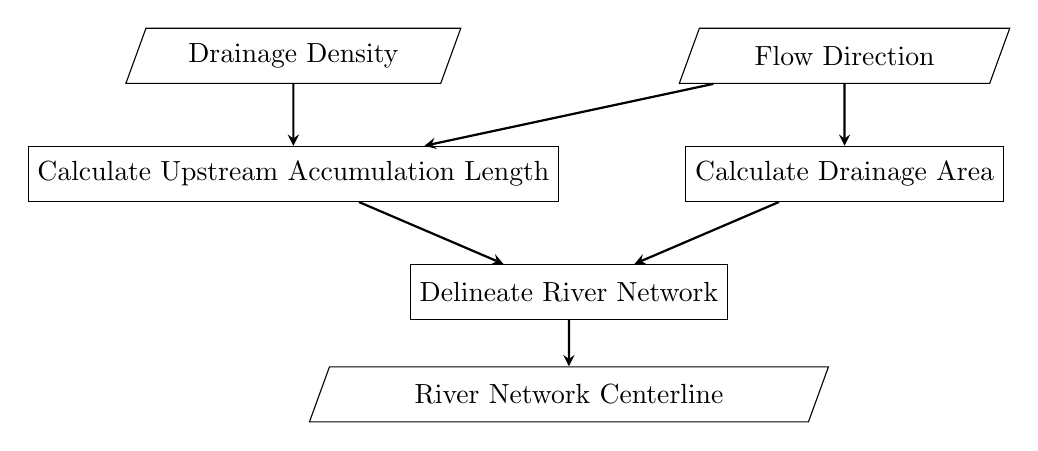
\begin{tikzpicture}
    \tikzstyle{startstop} = [rectangle, rounded corners, minimum width=3cm, minimum height=0.7cm,text centered, draw=black]
    \tikzstyle{io} = [trapezium, trapezium left angle=70, trapezium right angle=110, minimum width=2cm, minimum height=0.7cm, text centered, draw=black]
    \tikzstyle{process} = [rectangle, minimum width=3cm, minimum height=0.7cm, text centered, draw=black]
    \tikzstyle{decision} = [diamond, minimum width=3cm, minimum height=1cm, text centered, draw=black]
    \tikzstyle{arrow} = [thick,->,>=stealth]

    \node (dd) [io] {Drainage Density};
    \node (d8) [io, right of=dd, xshift=6cm] {Flow Direction};
    \node (upstream) [process, below of=dd, yshift=-0.5cm] {Calculate Upstream Accumulation Length};
    \node (drainage) [process, right of=upstream, below of=d8, xshift=-1cm, yshift=-0.5cm] {Calculate Drainage Area};
    \node (delineation) [process, below of=upstream, yshift=-0.5cm, xshift=3.5cm] {Delineate River Network};
    \node (output) [io, below of=delineation, yshift=-0.3cm, xshift=0cm] {River Network Centerline};

    \draw [arrow] (dd) -- (upstream);
    \draw [arrow] (d8) -- (upstream);
    \draw [arrow] (d8) -- (drainage);
    \draw [arrow] (upstream) -- (delineation);
    \draw [arrow] (drainage) -- (delineation);
    \draw [arrow] (delineation) -- (output);
  \end{tikzpicture}
  \caption{Flowchart illustrating the steps of the density-preserving river network delineation algorithm, including calculation of upstream accumulation length, drainage area, and final river network delineation.\label{fig:workflow}}
\end{figure}

\subsection{Upstream Accumulation Length}
\label{sec:upstream}

In this section, we first introduce the definition of upstream accumulation length. Then, we show how to calculate the upstream accumulation length using drainage density. Third, we prove that, given the flow direction, the upstream accumulation length is mathematically equivalent to drainage area by establishing the formula for inversing drainage density from upstream accumulation length. Finally, we present a fast algorithm to calculate the upstream accumulation length with O(N) time complexity.

As illustrated in Figure~\ref{fig:upstream}, the upstream accumulation length for a grid cell (Point O) is defined as the total length of river segments (i.e., segments A, B, and C) that lie within the catchment of the grid cell. This can be expressed mathematically as:
\begin{equation}
  \boldsymbol{L} = \int_{l \in \mathrm{Catchment}} \mathrm{d}l,
  \label{eq:upstream}
\end{equation}
where $\boldsymbol{L}$ represents the upstream accumulation length for the grid cell, $\mathrm{Catchment}$ denotes the catchment area of the grid cell, and $l$ is the length of the river segments within the catchment.

Equation~\ref{eq:upstream} can be rewritten using the definition of drainage density ($\boldsymbol{D} = \frac{\mathrm{d}l}{\mathrm{d}A}$) as follows:
\begin{equation}
  \boldsymbol{L} = \int_{A \in \mathrm{Catchment}} \frac{\mathrm{d}l}{\mathrm{d}A} \mathrm{d}A = \int_{A \in \mathrm{Catchment}} \boldsymbol{D} \, \mathrm{d}A,
  \label{eq:upstream_density}
\end{equation}
where $\mathrm{d}A$ denotes an infinitesimal area within the catchment and $\mathrm{d}l$ denotes the length of the river segments within the infinitesimal area. The equation states that the upstream accumulation length is equal to the integral of the drainage density over the area of the catchment. In other words, if we have two-dimensional drainage density data and know the catchment of every grid cell over the area (which is feasible given flow direction), we can calculate a two-dimensional upstream accumulation length at every grid cell using Equation~\ref{eq:upstream_density}.

Furthermore, given flow direction, upstream accumulation length and drainage density have a strictly one-to-one relationship. We can not only precisely estimate upstream accumulation length from drainage density (Equation~\ref{eq:upstream_density}), but also vice versa. The formula for calculating drainage density from upstream accumulation length can be derived by differentiating Equation~\ref{eq:upstream_density} as follows:
\begin{equation}
  \boldsymbol{D} = \frac{\mathrm{d}\boldsymbol{L}}{\mathrm{d}A} \text{.}
  \label{eq:density_upstream}
\end{equation}
This equation states that the drainage density of a grid cell is equal to the increase in upstream accumulation length divided by the area of the grid cell. The increase in upstream accumulation length can be estimated as the difference between the upstream accumulation length of a grid cell and the sum of the upstream accumulation length of the grid cell's donor cells. This one-to-one relationship between upstream accumulation length and drainage density is valid at any point of a two-dimensional domain.

\begin{figure}[H]
  \centering
  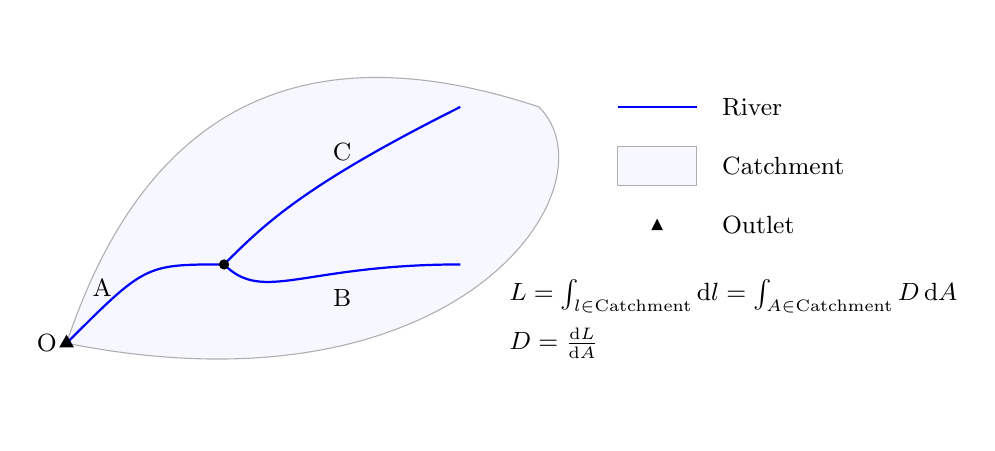
\begin{tikzpicture}[
      cell/.style={rectangle, draw, minimum size=1cm, font=\small},
      label/.style={font=\small}
    ]
    \tikzstyle{outlet} = [thick, fill=black]
    \tikzstyle{river} = [thick, blue]
    \tikzstyle{arrow} = [thick,->,>=stealth]
    \tikzstyle{catchment} = [draw=black, fill=blue!10, opacity=0.3]

    % Draw outer catchment
    \draw[catchment] (0, 0) .. controls (1, 3) and (3, 4) .. (6, 3) .. controls (7, 2) and (5, -1) .. (0, 0);

    % Draw river centerline A
    \draw[river] (0, 0) .. controls (1, 1) .. (2, 1);
    \node[label, left] at (0.7, 0.7) {A};

    % Draw river centerline B
    \draw[river] (2, 1) .. controls (2.5, 0.5) and (3, 1) .. (5, 1);
    \node[label, below] at (3.5, 0.8) {B};

    % Draw river centerline C
    \draw[river] (2, 1) .. controls (2.5, 1.5) and (3, 2) .. (5, 3);
    \node[label, above] at (3.5, 2.2) {C};

    % Draw outlets
    \draw[outlet] (0, 0) ++(-0.07,-0.04) -- ++(0.14,0) -- ++(-0.07,0.12) -- cycle;
    \node[label, left] at (0, 0) {O};

    \draw[outlet] (2.00,1.00) circle(0.05);

    % Add legend
    \draw[river] (7, 3) -- ++(1, 0);
    \node[label, right] at (8.2, 3) {River};
    \draw[catchment] (7, 2) rectangle ++(1, 0.5);
    \node[label, right] at (8.2, 2.25) {Catchment};
    \draw[outlet] (7.45, 1.45) -- ++(0.1, 0) -- ++(-0.05, 0.1) -- cycle;
    \node[label, right] at (8.2, 1.5) {Outlet};

    \node[label, right] at (5.5, 0.6) {$\boldsymbol{L} = \int_{l \in \mathrm{Catchment}} \mathrm{d}l = \int_{A \in \mathrm{Catchment}} \boldsymbol{D} \, \mathrm{d}A$};
    \node[label, right] at (5.5, 0) {$\boldsymbol{D} = \frac{\mathrm{d}\boldsymbol{L}}{\mathrm{d}A}$};
  \end{tikzpicture}
  \caption{Illustration of upstream accumulation length. Triangle symbols denote points in the study domain. The polygon represents the catchment of a point. Blue lines represent the river segments within the catchment. The upstream accumulation length ($\boldsymbol{L}$) is defined at the point, representing the total length of all the rivers within the catchment of the point. The symbol  $\boldsymbol{D}$ represents drainage density. \label{fig:upstream}}
\end{figure}

Given flow direction and drainage density, the calculation of upstream accumulation length can be performed efficiently. Inspired by the work of \citet{zhou2019FES}, we propose an algorithm to calculate the upstream accumulation length with O(N) time complexity. Algorithm~\ref{alg:upstream} depicts the pseudocode. In the algorithm, we define three types of grid cells: (1) source cells, (2) intersection cells, and (3) interior cells. The number of donor cells for source cells is 0, for intersection cells is greater than 1, and for interior cells is 1. The algorithm starts from the source cells and iteratively calculates the upstream accumulation length downstream until an intersection cell is encountered. The number of donor cells for the encountered intersection cell is then decreased by 1. The algorithm continues until all source cells are processed. Similar to \citet{zhou2019FES}, every grid cell is processed at most $n$ times, where $n$ is the maximum number of donor cells for a grid cell. Consequently, the time complexity of the algorithm is O(N), where N is the number of grid cells in the study area.

\begin{algorithm}[H]
  \caption{Algorithm for calculating upstream accumulation length. \label{alg:upstream}}
  \SetKwFor{Loop}{loop}{}{end}
  \KwIn{Two-dimensional flow direction ($\boldsymbol{F}$) and drainage density ($\boldsymbol{D}$)}
  \KwOut{Two-dimensional upstream flow accumulation length ($\boldsymbol{L}$) for each grid cell}
  \tcc{Count the number of upstream (donor) cells for each cell}
  Let $n$ be a two-dimensional array of the same size as $\boldsymbol{F}$, filled by zeros\;
  \ForEach{\normalfont{grid cell $(i, j)$ in the study area}}{
    Check the flow direction of $(i, j)$, identify the downstream grid cell $(i', j')$\;
    $n(i', j') = n(i', j') + 1$\;
  }
  \tcc{Find the source cells}
  Let $S$ be a stack of grid cell indices\;
  \ForEach{\normalfont{grid cell $(i, j)$ in the study area}}{
    \If{$n(i, j) = 0$}{
      Push $(i, j)$ to $S$\;
    }
  }
  \tcc{Initialize $\boldsymbol{L}$}
  Let $\boldsymbol{L}$ be a two-dimensional array of the same size as $\boldsymbol{F}$\;
  \ForEach{\normalfont{grid cell $(i, j)$ in the study area}}{
    $\boldsymbol{L}(i, j) = \boldsymbol{D}(i, j) \times A(i, j)$, where $A(i,j)$ is the grid cell area\;
  }
  \tcc{Propagate length from sources downstream}
  \While{$S$ is not empty}{
    Pop $(i, j)$ from $S$\;
    \While{\normalfont{Check the flow direction $\boldsymbol{F}$, if $(i,j)$ has a downstream cell $(i',j')$}}{
      $\boldsymbol{L}(i',j') = \boldsymbol{L}(i',j') + \boldsymbol{L}(i,j)$\;
      \If{$n(i',j') >= 2$} {
        $n(i',j') = n(i',j') - 1$\;
        Break\;
      }
      \Else{
        Let $(i,j) \leftarrow (i',j')$\;
      }
    }
  }
\end{algorithm}

\subsection{River Network Delineation with Upstream Accumulation Length}
\label{sec:network}

The key idea of our proposed algorithm is to transform drainage density into upstream accumulation length and to use the upstream accumulation length to delineate river networks. Since the upstream accumulation length and drainage density are mathematically equivalent, if the upstream accumulation length of every grid cell in the delineated river network matches the observed value, the drainage density of the delineated river network will also match the observed value at any point of a two-dimensional study area.

However, achieving this target exactly is computationally demanding. We can slightly relax the target and restate the objective of this study as follows: match the upstream accumulation length at every catchment outlet with the observed value. This relaxation significantly reduces the computational burden. Meanwhile, if the target is achieved, the average drainage density within every catchment of the delineated river network will also match the catchment-averaged observed value. This characteristic represents a substantial improvement over the existing methods discussed in the Introduction.

The delineation with the relaxed objective can be efficiently implemented using a divide-and-conquer strategy. Using Figure~\ref{fig:divide-conquer} as an illustration, the algorithm starts from the outlets of the whole domain (Outlet A in Figure~\ref{fig:divide-conquer}) and iteratively grows the centerlines of the river network (blue lines) by adding grid cells. If a bifurcation is encountered, the algorithm splits the river network into two or more parts (three parts in Figure~\ref{fig:divide-conquer}). A bifurcation point (the red point) is defined as a grid cell that lies on the existing centerline and has two or more donor cells that flow from existing centerlines into it. The donor cells of the bifurcation point (Outlets B and C) are then identified using flow direction. These donor cells serve as the outlets of the upstream catchments. The newly identified outlets split the river network into parts, each with a river segment (River A, B, and C) and a corresponding catchment (Catchment A, B, and C).

The algorithm calculates the expected length for each river segment based on the upstream accumulation length. If a reach has no upstreams (Rivers B and C), the expected length of the reach is the upstream accumulation length at its outlet (Outlets B and C). If a reach has upstreams (River A), the expected length is the upstream accumulation length at its outlet (Outlet A) minus the sum of the upstream accumulation lengths of all its upstreams at their outlets (Outlets B and C). The algorithm grows each river segment by adding grid cells and repeats the growing process until the length of every reach is greater than or equal to the expected length. When the iteration stops, the upstream accumulation length at every catchment outlet is equal to the observed value.

In Figure~\ref{fig:divide-conquer}, if the upstream accumulation length of the delineated network is the same as the observed value at Outlets B and C, the drainage density within Catchments B and C must match the observed drainage density. Since the upstream accumulation length at Outlet A is equal to the sum of the lengths of Rivers A, B, and C, if the expected length of River A is also achieved, the upstream accumulation length at Outlet A is equal to the observed value. Consequently, the drainage density within the combined catchments A, B, and C must also match the observed drainage density. Given that the drainage density within Catchments B and C is already equal to the observed value, the drainage density within Catchment A must also match the observed value. In this case, the drainage density within every catchment of the delineated river network is equal to the observed value.

The last piece of the algorithm is how to add grid cells to grow the river segments. There are certainly many ways to do this. We would like to keep our algorithm compatible with existing critical drainage area-based river network delineation algorithms. In critical drainage area-based algorithms, grid cells on the delineated rivers always have a larger drainage area value than those not delineated as rivers. Based on this observation, we grow the rivers by adding one grid cell at a time. The added grid cell is the one with the largest drainage area value among the neighbors of the delineated centerlines that flow into the centerlines. In this way, we ensure that the grid cells on the delineated centerlines always have a larger drainage area value than those not delineated as centerlines. This is the same idea as in critical drainage area-based algorithms.

\begin{figure}[H]
  \centering
  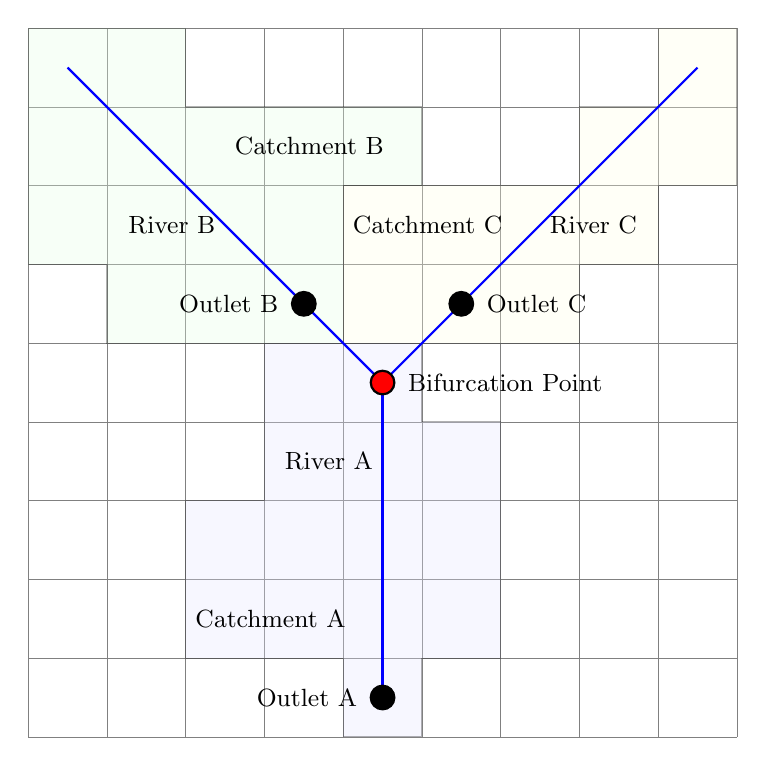
\begin{tikzpicture}[
      grid/.style={gray, very thin},
      cell/.style={rectangle, draw, minimum size=0.8cm, font=\small},
      river/.style={thick, blue},
      outlet/.style={thick, fill=black},
      bifurcation/.style={thick, fill=red},
      catchmentA/.style={draw=black, fill=blue!10, opacity=0.3},
      catchmentB/.style={draw=black, fill=green!10, opacity=0.3},
      catchmentC/.style={draw=black, fill=yellow!10, opacity=0.3},
      label/.style={font=\small}
    ]

    % Draw grid
    \draw[grid] (0, 0) grid (9, 9);

    % Draw catchment areas
    % Catchment for Reach A
    \draw[catchmentA] (4, 0) -- (5, 0) -- (5, 1) -- (6,1) -- (6, 4) -- (5, 4) -- (5, 5) -- (4, 5) -- (3, 5)  -- (3, 3) -- (2, 3) -- (2, 1) -- (4, 1) -- cycle;

    % Catchment for Reach B
    \draw[catchmentB] (1, 5) -- (4, 5) -- (4, 7) -- (5, 7) -- (5, 8) -- (2, 8) -- (2, 9) -- (0, 9) -- (0, 6) -- (1, 6) -- cycle;

    % Catchment for Reach C
    \draw[catchmentC] (4, 5) -- (7, 5) -- (7, 6) -- (8, 6) -- (8, 7) -- (9, 7) -- (9, 9) -- (8, 9) -- (8, 8) -- (7, 8) -- (7, 7) -- (4, 7) -- cycle;

    % Draw river centerlines (connecting centers of grid cells)
    \draw[river] (4.5, 0.5) -- (4.5, 4.5);
    \draw[river] (4.5, 4.5) -- (0.5, 8.5);
    \draw[river] (4.5, 4.5) -- (8.5, 8.5);

    % Draw outlets
    \draw[outlet] (4.5, 0.5) circle(0.15);
    \node[label, left] at (4.3, 0.5) {Outlet A};
    \draw[outlet] (3.5, 5.5) circle(0.15);
    \node[label, left] at (3.3, 5.5) {Outlet B};
    \draw[outlet] (5.5, 5.5) circle(0.15);
    \node[label, right] at (5.7, 5.5) {Outlet C};

    % Draw bifurcation point
    \draw[bifurcation] (4.5, 4.5) circle(0.15);
    \node[label, right] at (4.7, 4.5) {Bifurcation Point};

    % Label reaches
    \node[label, left] at (4.5, 3.5) {River A};
    \node[label, left] at (2.5, 6.5) {River B};
    \node[label, right] at (6.5, 6.5) {River C};

    % Catchment labels
    \node[label, right] at (2, 1.5) {Catchment A};
    \node[label, right] at (2.5, 7.5) {Catchment B};
    \node[label, right] at (4, 6.5) {Catchment C};

  \end{tikzpicture}
  \caption{Divide-and-conquer strategy for river network delineation using upstream accumulation length. The algorithm grows rivers to expected lengths independently within the three catchments. Blue lines denote the rivers. Grid cells filled with different colors denote the catchments of different rivers. Black dots denote the outlets of each catchment. \label{fig:divide-conquer}}
\end{figure}

Algorithm~\ref{alg:algorithm} shows pseudocode for the density-preserving river network delineation algorithm. The algorithm utilizes two queues: the Open queue, which is a temporary store of partially delineated rivers, and the Lines queue, which stores the finalized rivers. The algorithm grows each river in the Open queue. If the length of a river is greater than or equal to the expected length, the river is finalized and moved to the Lines queue. If a bifurcating condition is encountered, the algorithm divides the river into parts, as illustrated in Figure~\ref{fig:divide-conquer}, and puts the parts back into the Open queue.

The algorithm is efficient. The divide-and-conquer strategy ensures that the river-growing process focuses on a specific reach and its neighboring grid cells at a time, without having to consider the entire study domain. This locality is especially important when dealing with large domains such as at the scale of a country, a continent, or even the globe.

\begin{algorithm}[H]
  \caption{Density-preserving river network delineation algorithm.\label{alg:algorithm}}
  \SetKwFor{Loop}{loop}{}{end}
  \KwIn{Two-dimensional flow direction ($\boldsymbol{F}$), drainage area ($\boldsymbol{A}$), and upstream accumulation length ($\boldsymbol{L}$)}
  \KwOut{$Lines$ is a list of rivers, each represented by a list of grid cell indicies}
  \tcc{Initialization of the delineation}
  Let $Open$ be an empty queue of lists of grid cell indicies\;
  \ForEach{\normalfont{outlet $(i, j)$ in the study area}}{
    \If{$\boldsymbol{A}(i, j) > 0$}{
      $Open$.push(single-element list $[(i, j),]$)\;
    }
  }
  \tcc{Delineation of river centerlines}
  \While{\normalfont{$Open$ is not empty}}{
    $L$ = $Open$.pop()\;
    \If{$L$ \normalfont{has no upstreams}} {
      Let the expected length $l \leftarrow \boldsymbol{L}(i, j)$, where $(i, j)$ is the last grid cell of $L$\;
    }\Else{
      Let the expected length $l \leftarrow \boldsymbol{L}(i, j) - \sum \boldsymbol{L}(i', j')$, where $(i ,j)$ is the last grid cell of $L$, $(i', j')$ is the last grid cell of the upstream of $L$\;
    }
    \Loop{}{
      Let $N$ be a set of grid cells. Each of $N$: (1) is the neighbor of $L$, (2) flow into $L$, and (3) have not been included in any line in $Lines$ or in $Open$\;
      \If{\normalfont{Length of} $L \geq l$ \textbf{or} $N$ is empty}{
        $Lines$.append($L$)\;
        break\;
      }
      Find the grid cell $(i_2, j_2)$ in $N$ that has the largest $\boldsymbol{A}$\;
      Find $(i', j')$ that is the grid cell that $(i_2, j_2)$ flows to, $(i_1, j_1)$ is the grid cell in $L$ that also flows to $(i', j')$\;
      \uIf{\normalfont{$(i', j')$ is the last grid cell of $L$}}{
        $L$.append($(i_2, j_2)$)\;
      }
      \Else{
        \tcc{Bifurcation}
        Split $L$ into two sub-list: $L_1$ is the list before $(i', j')$ (inclusive) and $L_2$ is the one after $(i', j')$ (exclusive)\;
        $Open$.push($L_1$)\;
        $Open$.push($L_2$)\;
        $Open$.push(one-element list [$(i_1, j_1),$])\;
        break\;
      }
    }
  }
\end{algorithm}

\subsection{Avoidance of Short River Segments}
\label{sec:short}

The algorithm shown in Algorithm~\ref{alg:algorithm} strictly preserves the observed drainage density for every catchment of the delineated river network. However, the algorithm often produces a large number of short river segments. These short river segments are not only difficult to represent in hydrodynamic simulations but also have a negligible impact on the overall drainage density. Algorithm~\ref{alg:algorithm_improve} shows an improved algorithm tailored for hydrodynamic simulations. Two thresholds are introduced in the algorithm: one for the minimum length of river segments ($l_\mathrm{cr}$, line 24 in Algorithm~\ref{alg:algorithm_improve}) and the other for the minimum drainage area ($A_\mathrm{cr}$, line 17 in Algorithm~\ref{alg:algorithm_improve}). The former is used to avoid overly short river segments on mainstreams, while the latter is used to avoid overly short river segments on head waters.

\begin{algorithm}[H]
  \caption{Density-preserving river network delineation algorithm with thresholds for river segment length and drainage area.\label{alg:algorithm_improve}}
  \SetKwFor{Loop}{loop}{}{end}
  \KwIn{Two-dimensional flow direction ($\boldsymbol{F}$), drainage area ($\boldsymbol{A}$), upstream accumulation length ($\boldsymbol{L}$), critical drainage area ($A_{\mathrm{cr}}$), and critical length ($l_{\mathrm{cr}}$)}
  \KwOut{$Lines$ is a list of centerlines, each represented by a list of grid cell indicies}
  \tcc{Initialization of the delineation}
  Let $Open$ be an empty queue of lists of grid cell indicies\;
  \ForEach{\normalfont{outlet $(i, j)$ in the study area}}{
    \If{$\boldsymbol{A}(i, j) > 0$}{
      $Open$.push(single-element list $[(i, j),]$)\;
    }
  }
  \tcc{Delineation of river centerlines}
  \While{\normalfont{$Open$ is not empty}}{
    $L$ = $Open$.pop()\;
    \If{$L$ \normalfont{has no upstreams}} {
      Let the expected length $l \leftarrow \boldsymbol{L}(i, j)$, where $(i, j)$ is the last grid cell of $L$\;
    }\Else{
      Let the expected length $l \leftarrow \boldsymbol{L}(i, j) - \sum \boldsymbol{L}(i', j')$, where $(i ,j)$ is the last grid cell of $L$, $(i', j')$ is the last grid cell of the upstream of $L$\;
    }
    \Loop{}{
      Let $N$ be a set of grid cells. Each of $N$: (1) is the neighbor of $L$, (2) flow into $L$, and (3) have not been included in any line in $Lines$ or in $Open$\;
      \If{\normalfont{Length of} $L \geq l$ \textbf{or} $N$ is empty}{
        $Lines$.append($L$)\;
        break\;
      }
      Find the grid cell $(i_2, j_2)$ in $N$ that has the largest $\boldsymbol{A}$\;
      \If{$\boldsymbol{A}(i_2, j_2) \leq A_{\mathrm{cr}}$}{
        $Lines$.append($L$)\;
        break\;
      }
      Find $(i', j')$ that is the grid cell that $(i_2, j_2)$ flows to, $(i_1, j_1)$ is the grid cell in $L$ that also flows to $(i', j')$\;
      \uIf{\normalfont{$(i', j')$ is the last grid cell of $L$}}{
        $L$.append($(i_2, j_2)$)\;
      }
      \Else{
        \tcc{Bifurcation}
        \If{\normalfont{Length of} $L < l_{\mathrm{cr}}$}{
          $Lines$.append($L$)\;
          break\;
        }
        Split $L$ into two sub-list: $L_1$ is the list before $(i', j')$ (inclusive) and $L_2$ is the one after $(i', j')$ (exclusive)\;
        $Open$.push($L_1$)\;
        $Open$.push($L_2$)\;
        $Open$.push(one-element list [$(i_1, j_1),$])\;
        break\;
      }
    }
  }
\end{algorithm}

\section{Experimental Setup}
\label{sec:experiment}

We test the proposed algorithm using two cases: a synthetic case and a real-world case. The synthetic case is designed to demonstrate the steps of the algorithm and to show its compatibility with the critical drainage area-based algorithm. The real-world case is designed to demonstrate the computational efficiency and effectiveness of the proposed algorithm in delineating river networks over large domains.

The synthetic case is a 4\texttimes{}4 grid with a grid size of 1\texttimes{}1. Figure~\ref{fig:example}b show the flow direction and drainage area, respectively. A river network is first delineated using the critical drainage area-based algorithm with a threshold of 4, as shown in Figure~\ref{fig:example}c. This river network is used as the synthetic truth. Drainage density is calculated from this network. We then delineate the river network using the proposed algorithm to check whether the proposed algorithm can produce the same river network shown in Figure~\ref{fig:example}c.

The real-world case involves delineating the river network over the Chinese Mainland. The MERIT-Hydro flow direction dataset \citep{yamazaki2019WRR} is used in this case. MERIT-Hydro is a global 3-arc-second (approximately 90 m) resolution dataset derived from the MERIT DEM \citep{yamazaki2017GRL}. This dataset has been widely used in hydrodynamic simulations \citep{yang2021BAMS}. \citet{lin2021SD} have shown that the river network delineated from the MERIT-Hydro flow direction dataset has high accuracy in terms of centerline position. The drainage density dataset used in this case is produced from the Third National Land Resources Survey of China \citep{zhang2024CDB}. The dataset covers the entire Chinese Mainland at a spatial resolution of 1 km. We bilinearly interpolated the 1-km drainage density data to the 90-m MERIT-Hydro grid. To ensure the delineated river network is continuous, we slightly extended the boundary of the study area outside the Chinese Mainland. In these extended areas, there is no surveyed drainage density data. The drainage density is estimated using a river network delineated from the MERIT-Hydro dataset and the critical drainage area-based method with a threshold of 1 km\textsuperscript{2}.

\section{Results}
\label{sec:results}

\subsection{The Synthetic Case}
\label{sec:test_case}

Figure~\ref{fig:example}d shows the drainage density calculated from Figure~\ref{fig:example}c. Note that the river length at each grid cell is calculated as the total length of the river segments connecting the grid cell center to the centers of its upstream cells. This calculation differs slightly from survey data or imagery-based data. If the grid cell is small (i.e., a typical grid cell is smaller than 100 m\texttimes{}100 m), the difference is negligible. Figure~\ref{fig:example}e shows the total upstream river length calculated according to the algorithm described in Algorithm~\ref{alg:upstream}.

The last row of Figure~\ref{fig:example} reveals the delineation process. Figure~\ref{fig:example}f shows the state after initialization. The $Open$ queue contains the grid cells at the outlets of the whole domain. After initialization, a centerline is grown from the outlet by adding the grid cell with the largest drainage area value in the neighborhood of the already delineated centerlines. This process is repeated until a bifurcating condition is encountered. Figure~\ref{fig:example}g shows the bifurcating condition, where the solid lines denote the already delineated rivers and the dashed line connects the grid cell with the largest drainage area value.

As the grid cell with the largest drainage area value (denoted by the dot connected by the dashed line) does not flow to the head of the river, the river is split into two parts, denoted by the magenta and black lines in Figure~\ref{fig:example}h. The parts and the grid cell with the largest drainage area (i.e., the green line) are then added to the $Open$ queue for further delineation. In this simple case, the lengths of all three centerlines are already greater than or equal to the expected river length at this stage, as described in Algorithm~\ref{alg:algorithm}, so the algorithm terminates.

In this synthetic case, the river network delineated using our proposed algorithm (Figure~\ref{fig:example}h) is identical to the one delineated using the critical drainage area-based method (Figure~\ref{fig:example}c). This demonstrates that our proposed algorithm produces the same results as the widely-used critical drainage area-based methods when using the same drainage density. The key difference lies in the input requirements: our algorithm utilizes two-dimensional drainage density (Figure~\ref{fig:example}d) as an input parameter, whereas the critical drainage area-based method lacks a priori information on drainage density and instead relies on an empirical parameter of critical drainage area.

\begin{figure}[H]
  \subfloat[Flow direction]{
    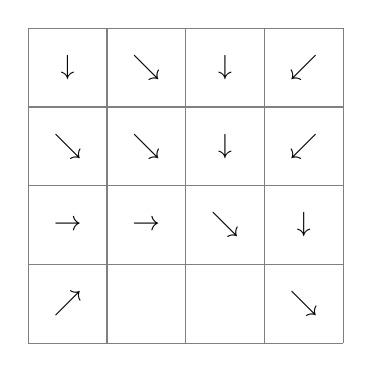
\begin{tikzpicture}
      \draw[step=1cm,color=gray] (-2,-2) grid (2,2);

      \node at (-1.5,+1.5) {$\downarrow$};
      \node at (-0.5,+1.5) {$\searrow$};
      \node at (+0.5,+1.5) {$\downarrow$};
      \node at (+1.5,+1.5) {$\swarrow$};

      \node at (-1.5,+0.5) {$\searrow$};
      \node at (-0.5,+0.5) {$\searrow$};
      \node at (+0.5,+0.5) {$\downarrow$};
      \node at (+1.5,+0.5) {$\swarrow$};

      \node at (-1.5,-0.5) {$\rightarrow$};
      \node at (-0.5,-0.5) {$\rightarrow$};
      \node at (+0.5,-0.5) {$\searrow$};
      \node at (+1.5,-0.5) {$\downarrow$};

      \node at (-1.5,-1.5) {$\nearrow$};
      % \node at (-0.5,-1.5) {$\searrow$};
      % \node at (+0.5,-1.5) {$\downarrow$};
      \node at (+1.5,-1.5) {$\searrow$};
    \end{tikzpicture}
  }
  \subfloat[Drainage area]{
    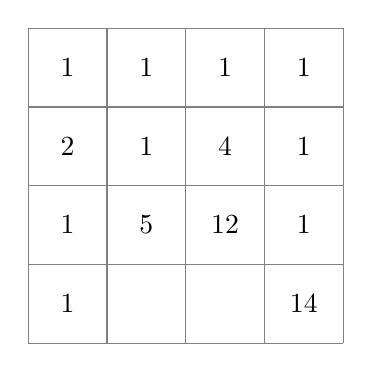
\begin{tikzpicture}
      \draw[step=1cm,color=gray] (-2,-2) grid (2,2);

      \node at (-1.5,+1.5) {$1$};
      \node at (-0.5,+1.5) {$1$};
      \node at (+0.5,+1.5) {$1$};
      \node at (+1.5,+1.5) {$1$};

      \node at (-1.5,+0.5) {$2$};
      \node at (-0.5,+0.5) {$1$};
      \node at (+0.5,+0.5) {$4$};
      \node at (+1.5,+0.5) {$1$};

      \node at (-1.5,-0.5) {$1$};
      \node at (-0.5,-0.5) {$5$};
      \node at (+0.5,-0.5) {$12$};
      \node at (+1.5,-0.5) {$1$};
      % ...
      \node at (-1.5,-1.5) {$1$};
      \node at (-0.5,-1.5) {};
      \node at (+0.5,-1.5) {};
      \node at (+1.5,-1.5) {$14$};
    \end{tikzpicture}
  }
  \subfloat[River centerline]{
    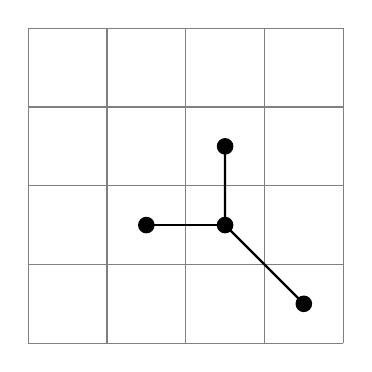
\begin{tikzpicture}
      \draw[step=1cm,color=gray] (-2,-2) grid (2,2);
      % Mark cells with flow accumulation ≥ 4 as red dots
      \fill[black] (0.5,0.5) circle (3pt);    % value 4
      \fill[black] (-0.5,-0.5) circle (3pt);  % value 5
      \fill[black] (0.5,-0.5) circle (3pt);   % value 12
      \fill[black] (1.5,-1.5) circle (3pt);   % value 14

      % Draw the main centerline along the highest accumulated path
      \draw[black,thick] (0.5,0.5) -- (0.5,-0.5) -- (1.5,-1.5);
      \draw[black,thick] (0.5,-0.5) -- (-0.5,-0.5);
    \end{tikzpicture}
  }

  \subfloat[Drainage density]{
    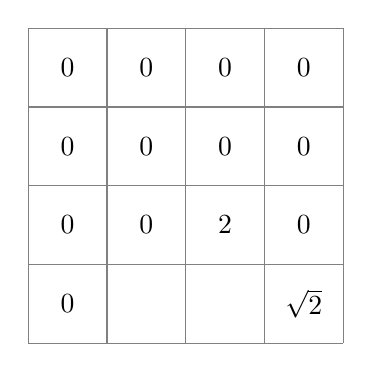
\begin{tikzpicture}
      \draw[step=1cm,color=gray] (-2,-2) grid (2,2);

      \node at (-1.5,+1.5) {$0$};
      \node at (-0.5,+1.5) {$0$};
      \node at (+0.5,+1.5) {$0$};
      \node at (+1.5,+1.5) {$0$};

      \node at (-1.5,+0.5) {$0$};
      \node at (-0.5,+0.5) {$0$};
      \node at (+0.5,+0.5) {$0$};
      \node at (+1.5,+0.5) {$0$};

      \node at (-1.5,-0.5) {$0$};
      \node at (-0.5,-0.5) {$0$};
      \node at (+0.5,-0.5) {$2$};
      \node at (+1.5,-0.5) {$0$};
      % ...
      \node at (-1.5,-1.5) {$0$};
      \node at (-0.5,-1.5) {};
      \node at (+0.5,-1.5) {};
      \node at (+1.5,-1.5) {$\sqrt{2}$};
    \end{tikzpicture}
  }
  \subfloat[Total upstream river length]{
    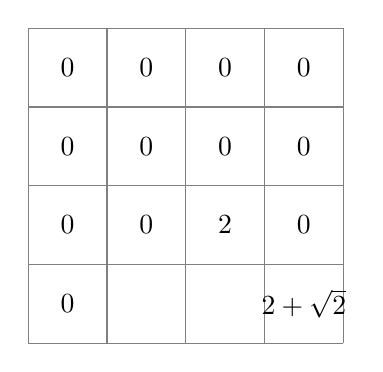
\begin{tikzpicture}
      \draw[step=1cm,color=gray] (-2,-2) grid (2,2);

      \node at (-1.5,+1.5) {$0$};
      \node at (-0.5,+1.5) {$0$};
      \node at (+0.5,+1.5) {$0$};
      \node at (+1.5,+1.5) {$0$};

      \node at (-1.5,+0.5) {$0$};
      \node at (-0.5,+0.5) {$0$};
      \node at (+0.5,+0.5) {$0$};
      \node at (+1.5,+0.5) {$0$};

      \node at (-1.5,-0.5) {$0$};
      \node at (-0.5,-0.5) {$0$};
      \node at (+0.5,-0.5) {$2$};
      \node at (+1.5,-0.5) {$0$};
      % ...
      \node at (-1.5,-1.5) {$0$};
      \node at (-0.5,-1.5) {};
      \node at (+0.5,-1.5) {};
      \node at (+1.5,-1.5) {$2 + \sqrt{2}$};
    \end{tikzpicture}
  }

  \subfloat[Initial state]{
    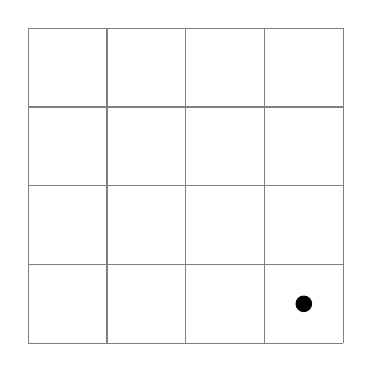
\begin{tikzpicture}
      \draw[step=1cm,color=gray] (-2,-2) grid (2,2);
      \fill[black] (1.5,-1.5) circle (3pt);   % value 14

    \end{tikzpicture}
  }
  \subfloat[Bifurcating condition]{
    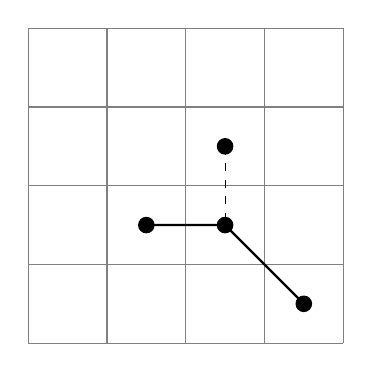
\begin{tikzpicture}
      \draw[step=1cm,color=gray] (-2,-2) grid (2,2);
      % Mark cells with flow accumulation ≥ 4 as red dots
      \fill[black] (0.5,0.5) circle (3pt);    % value 4
      \fill[black] (-0.5,-0.5) circle (3pt);  % value 5
      \fill[black] (0.5,-0.5) circle (3pt);   % value 12
      \fill[black] (1.5,-1.5) circle (3pt);   % value 14

      % Draw the main centerline along the highest accumulated path
      \draw[black,thick] (-0.5,-0.5) -- (0.5,-0.5) -- (1.5,-1.5);
      \draw[black,dashed] (0.5,0.5) -- (0.5,-0.5);
    \end{tikzpicture}
  }
  \subfloat[Bifurcated state]{
    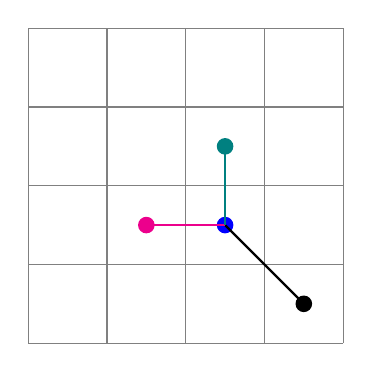
\begin{tikzpicture}
      \draw[step=1cm,color=gray] (-2,-2) grid (2,2);
      % Mark cells with flow accumulation ≥ 4 as red dots
      \fill[teal] (0.5,0.5) circle (3pt);    % value 4
      \fill[magenta] (-0.5,-0.5) circle (3pt);  % value 5
      \fill[blue] (0.5,-0.5) circle (3pt);   % value 12
      \fill[black] (1.5,-1.5) circle (3pt);   % value 14

      % Draw the main centerline along the highest accumulated path
      \draw[black,thick] (0.5,-0.5) -- (1.5,-1.5);
      \draw[magenta,thick] (-0.5,-0.5) -- (0.5,-0.5);
      \draw[teal,thick] (0.5,0.5) -- (0.5,-0.5);
    \end{tikzpicture}
  }
  \caption{An illustration of the density-preserving river network delineation algorithm. Panel (c) serves as the synthetic truth of the river network. \label{fig:example}}
\end{figure}

\subsection{The Real-World Case}

In the real-world case, we applied the improved algorithm shown in Algorithm~\ref{alg:algorithm_improve} to delineate the river network over the Chinese Mainland. The delineation was performed on the 90-m MERIT Hydro grids using a 0.5 km\textsuperscript{2} threshold for the minimum drainage area and a 0.5 km threshold for the minimum river segment length.

The delineation process was efficient, completing in less than 10 minutes using a single thread of an Apple M3 Max processor. This represents a substantially reduced computational burden compared to previous studies \citep{lin2021SD}. The efficiency is attributed to the divide-and-conquer strategy and the use of two-dimensional drainage density information as a priori input, rather than using it ad hoc in a trial-and-error process. The delineated river network consists of 2,314,986 river segments, which are available for download from \url{https://doi.org/10.57760/sciencedb.23487} (accessed on 2024-04-10).

\begin{figure}[H]
  \includegraphics[width=\textwidth]{china.png}
  \caption{A Chinese Mainland river network dataset delineated using the drainage density-preserving method.\label{fig:china}}
\end{figure}

Besides showing the efficiency, we also demonstrate the effectiveness of the proposed algorithm in capturing the variation of drainage density. Figure~\ref{fig:comparison} compares the river network delineation results in South Xinjiang, China. South Xinjiang is characterized by a variety of landscapes, including mountains and deserts. The drainage density varies significantly across the region, making it an ideal testbed for intercomparison. Figure~\ref{fig:comparison}a shows the river network delineated using the critical drainage area-based method with a threshold of 10 km\textsuperscript{2}. The river network appears nearly uniform across the region, failing to capture the variation in drainage density. Compared with satellite imagery, the river network is overly dense in the desert areas. Figure~\ref{fig:comparison}b shows the river network delineated using the drainage density-preserving method. The result is encouraging, not only representing the contrast in drainage density between the foothills and deserts, but also resolving rivers that flow across the desert. Figure~\ref{fig:comparison}c shows the Hydrological data and maps based on the Shuttle Elevation Derivatives at Multiple Scales (HydroSHEDS) river network dataset, while Figure~\ref{fig:comparison}d shows the MERIT-Vector river network dataset \citep{lin2021SD}. MERIT-Vector has a much denser network than HydroSHEDS and shows more variation in drainage density. However, they both produce overly dense river networks in the desert and show smaller variations between foothills and desert than Figure~\ref{fig:comparison}b. The comparison demonstrates that our proposed algorithm can effectively capture the variation in drainage density across the entire river network, a feature that existing publicly available datasets have not performed as well in.

In this study, we have not evaluated the position accuracy of the delineated river network centerline. Since we are using the same flow direction dataset as \citet{lin2021SD}, we expect that the river network delineated in this study will also achieve a similar level of centerline position accuracy as reported by \citet{lin2021SD}.

\begin{figure}[H]
  %\isPreprints{} % If the paper is ``preprints'', please uncomment this parenthesis.
    \subfloat[\centering 10 km\textsuperscript{2} drainage area threshold]{\includegraphics[width=8.0cm]{xinjiang-10km2.png}}
    %\hfill
    \subfloat[\centering The Drainage Density-Preserving Method]{\includegraphics[width=8.0cm]{xinjiang-thisalgorithm.png}}\\
    \subfloat[\centering HydroSHEDS]{\includegraphics[width=8.0cm]{xinjiang-hydroshed.png}}
    %\hfill
    \subfloat[\centering MERIT-Vector]{\includegraphics[width=8.0cm]{xinjiang-meritvector.png}}\\
    \subfloat[\centering Satellite Imagery]{\includegraphics[width=7.0cm]{xinjiang-satellite.png}}
    %\isPreprints{}{% This command is only used for ``preprints''.
  \end{adjustwidth}
  \caption{Comparison of the river network delineation results in South Xinjiang. (\textbf{a}) delineation with critical drainage area of 10 km\textsuperscript{2}, (\textbf{b}) delineation with the drainage density-preserving method, (\textbf{c}) the HydroSHED river network dataset, (\textbf{d}) the MERIT-Vector river network dataset, and (\textbf{e}) Satellite imagery.\label{fig:comparison}}
\end{figure}

\section{Discussion}
\label{sec:discussion}

The proposed algorithm uses two-dimensional drainage density as a priori information to delineate river networks, and the delineated river network can preserve the observed drainage density at every delineated catchment. This represents a significant improvement over existing methods, which often fail to capture the variation of drainage density across large domains. The capability of capturing the variation of drainage density is not limited to the spatial dimension but could also be extended to the temporal dimension. Given a time-varying drainage density dataset, the proposed algorithm can be used to delineate river networks that preserve the observed drainage density at every time step. Although we do not expect the algorithm to capture fragmented rivers, it is still able to represent the extension and retreat of headwaters. Such studies would be useful for understanding the changes in non-perennial rivers and the impacts of climate change on river networks \cite{durighetto2022GRL, zanetti2024WRR, price2021GRL, messager2021N}.

However, the proposed algorithm is still subject to several limitations that are common to all DEM-based methods. First, the resolution of the input DEM significantly affects the delineation results \cite{mcmaster2002WRR}. A higher resolution DEM provides more accurate flow direction and drainage area information, would leading to a more accurate delineation of river networks. However, DEM-based methods discussed in this study have difficulties when the DEM resolution is too fine. As shown by \citet{bernard2022JGRES, costabile2024JH}, these methods, including the one proposed in this study, are not able to capture the morphology of rivers wider than the resolution. Special treatment of the river surface \cite{barnes2014CG} is necessary to adjust the DEM. Second, the delineated river network is affected by the accuracy of the input DEM and drainage density data. Dense vegetation in the tropics and steep terrain at the edge of mountains can introduce errors in the DEMs, which can propagate to the delineated river network. In this study, we used the MERIT-Hydro dataset, which is produced by correcting multiple errors in DEMs, including the impacts of vegetation. However, the impacts of errors in drainage density data are still unknown. We leave the investigation of drainage density's impact for future research to keep this paper focused and concise. Third, the delineated river network represents mere line skeletons without width information. For use in large-domain hydrodynamic simulations, the cross-section of the rivers is parameterized using simple geometry and calibratable geometric parameters \cite{read2023JAWRA}. This approach often faces difficulties in representing floodplains accurately. Two-dimensional hydraulic simulations on DEMs show potential to address these limitations. However, the computational cost hinders the application of two-dimensional hydraulic simulations on large domains, like the Chinese Mainland presented in this study.

\section{Conclusions}
\label{sec:conclusion}

This study introduces a novel river network delineation method that preserves observed drainage density across the entire river network. The method is based on a novel concept named upstream accumulation length, which is calculated using flow direction and drainage density. The delineation algorithm is designed to be compatible with critical drainage area-based methods, allowing for the preservation of observed drainage density in every single catchment of the river network.

The proposed algorithm was applied to the Chinese Mainland, utilizing the MERIT-Hydro flow direction dataset and a kilometer-resolution drainage density dataset produced from the Third National Land Resources Survey of China. The resulting river network dataset is segmented into nearly uniform lengths of approximately one kilometer, providing a critical foundation for the development of national-scale flood forecasting systems in the Chinese Mainland.

The proposed algorithm was tested on a synthetic case and a real-world case. The results from the synthetic case demonstrated that the proposed algorithm can produce the same river network as critical drainage area-based methods when using the same drainage density. The real-world case that to delineate the river network over Chinese Mainland showed that the proposed algorithm is both computationally efficient and effective in capturing the variation of drainage density. 2,314,986 river segments were delineated in less than 10 minutes on a single thread of an Apple M3 Max processor. The delineated river network was shown to be superior in capturing the variation of drainage density across the entire river network compared to existing publicly available datasets such as HydroSHEDS and MERIT-Vector.

The results are encouraging, since the method opens the possibility of combining aerial satellite imagery and DEMs to delineate river networks accurately on a global scale. This is particularly important, as only a few countries (e.g., the United States of America, the United Kingdom, France, and Australia) have manually maintained river network datasets. The vast majority of the world, including China, lacks such datasets. The proposed algorithm can be applied to delineate river networks in these regions, providing a valuable resource for hydrodynamic simulations and flood forecasting systems.

\vspace{6pt}

\authorcontributions{Conceptualization, H.Z.; methodology, H.Z.; software, H.Z.; validation, S.C. and H.Y.; formal analysis, S.C. and H.Y.; investigation, S.C. and H.Y.; resources, S.C., H.Y. and H.Z.; data curation, S.C. and H.Y.; writing---original draft preparation, S.C. and H.Y.; writing---review and editing, S.C., H.Y., and H.Z.; visualization, S.C. and H.Y.; supervision, H.Z.; project administration, H.Z.; funding acquisition, H.Z. All authors have read and agreed to the published version of the manuscript.}

\funding{This study is funded by China Three Gorges Corporation (contract Z532302035), the National Key Research and Development Program of China (2023YFF0805501), and the Natural Science Foundation of China (grants 42075165 and 42275178).}

\dataavailability{The MERIT-Hydro dataset was obtained from \url{https://hydro.iis.u-tokyo.ac.jp/~yamadai/MERIT_Hydro/} (accessed on 2024-11-10). The 1\,km Drainage Density Dataset in China (2022) was obtained from \url{https://doi.org/10.57760/sciencedb.16001} (accessed on 2024-11-10). The MERIT-Vector river network dataset was obtained from \url{https://doi.org/10.6084/m9.figshare.c.5052635.v1} (accessed on 2025-01-10). The HydroSHED river network dataset was obtained from \url{https://www.hydrosheds.org} (accessed on 2025-01-10). The delineated river network dataset in this study can be found on \url{https://doi.org/10.57760/sciencedb.23487} (accessed on 2024-04-10).}

\conflictsofinterest{Authors Heng Yang and Shuanglong Chen were employed by the China Three Gorges Corporation. The remaining author declares that the research was conducted in the absence of any commercial or financial relationships that could be construed as a potential conflict of interest.}

%\isPreprints{} % If the paper is ``preprints'', please uncomment this parenthesis.
  %\printendnotes[custom] % Un-comment to print a list of endnotes

  \reftitle{References}
  \bibliography{references.bib}

  \PublishersNote{}
  %\isPreprints{} % If the paper is ``preprints'', please uncomment this parenthesis.
\end{document}
